\section{Experiment Environment Setup}

\begin{itemize}
    \item \textbf{Host Operating System}:Arch Linux\footnote{Arch Linux is following a rolling-release model. The test running on both hosts and guests were the most recent systems available at the time of this report.}
    \item \textbf{Linux Kernel Version}: 5.14.14 with ZEN optimization
    \item \textbf{Hypervisor / Manager}: QEMU 5.2.0 / Libvirtd 7.8.0
    \item \textbf{Guest Operating System}: Arch Linux
\end{itemize}

\subsection*{Building QEMU}

The QEMU version provided by Arch Linux is 6.1.0, and as it is a rolling-release distribution, we need to downgrade it into an older version. To minimize clashes with original packages provided by distribution, and patch QEMU with system-specific options, we used the older version of the package build script to build QEMU.\footnote{The packaging script can be found  \textcolor{blue}{\href{https://github.com/archlinux/svntogit-packages/tree/3049c9e5bcef3221532391bc719d07e9a4386a25}{here}}.}

\begin{figure}[ht]
    \centering
    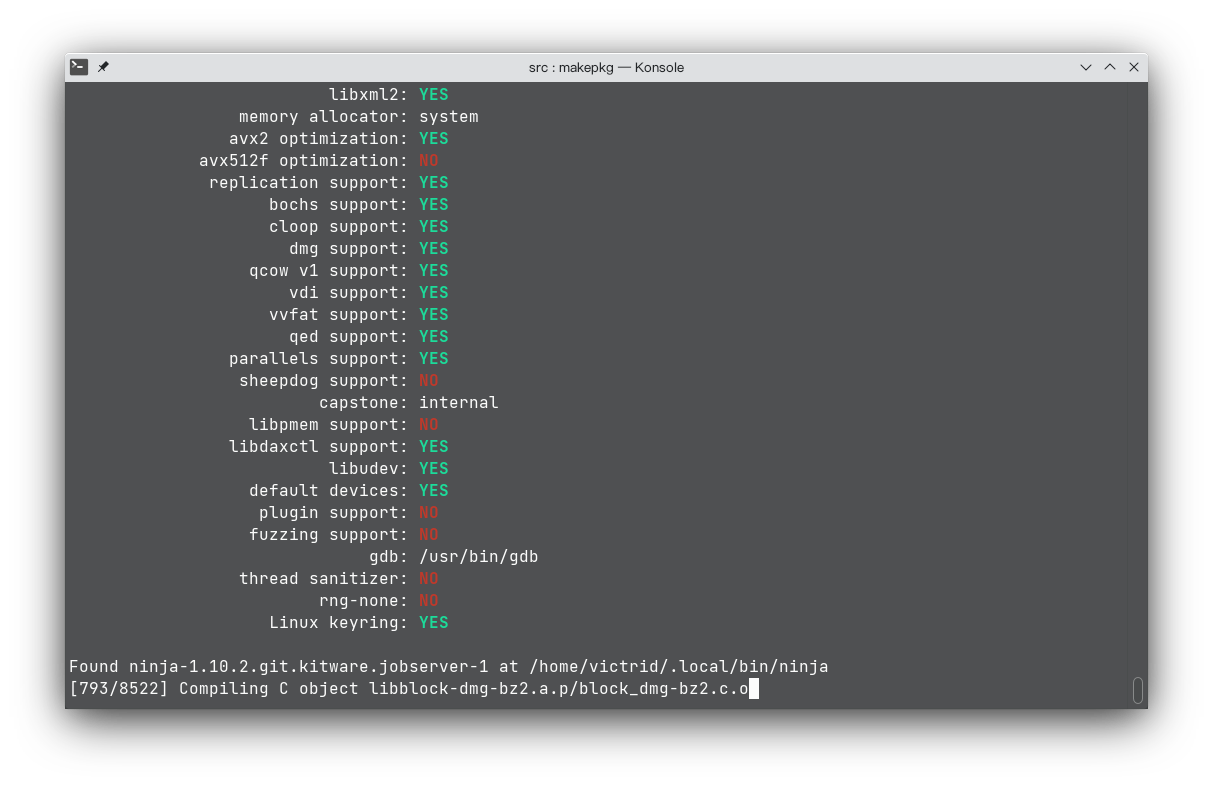
\includegraphics[width=0.7\textwidth]{images/compiling-qemu.png}
    \caption{Building QEMU}
    \label{fig:compile}
\end{figure}

\subsection*{Configuring Virtual Machine}

Although QEMU can be started from the command line, for a more structured presentation of the virtual machine configuration process, we use the virtual machine manager provided by Libvirtd to manage it.

Arch Linux provides a series of disk images of virtual machines with minimized systems pre-installed\footnote{The build can be found  \textcolor{blue}{\href{https://gitlab.archlinux.org/archlinux/arch-boxes/-/jobs/38089/artifacts/browse/output}{here}}.}. We use \texttt{ping} and \texttt{iperf} for testing various parameters of the network, where \texttt{iperf} is not included in the image, so it is also necessary to install \texttt{iperf} on the system.

\begin{figure}[ht]
    \centering
    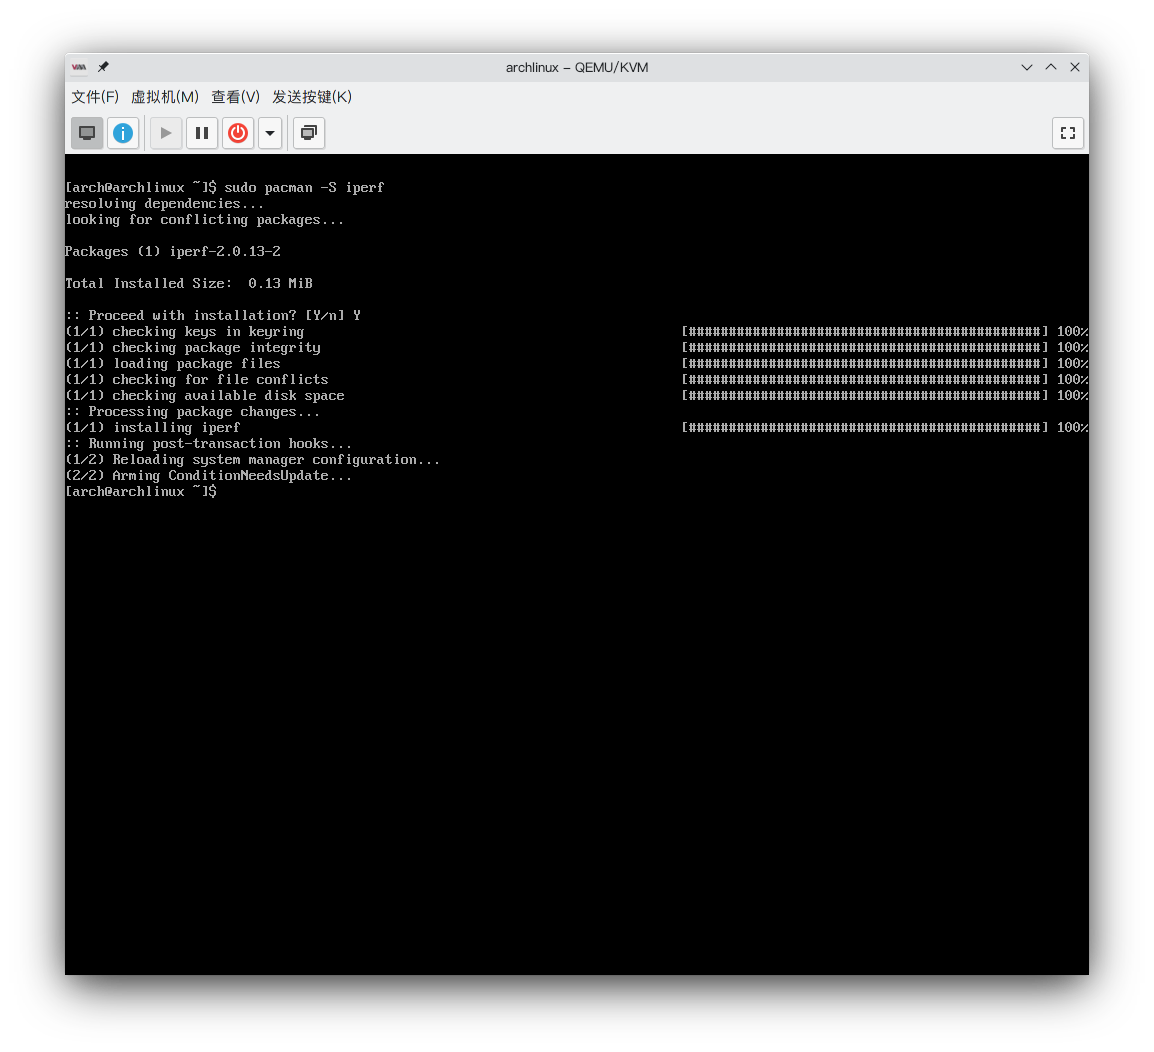
\includegraphics[width=0.8\textwidth]{images/install_iperf.png}
    \caption{Install iperf}
    \label{fig:compile}
\end{figure}

Virtual machines can be migrated quickly by replicating configurations, etc. By creating snapshots among each instance, different virtual machines can share the same base disk image.